% ColombiaMacro — presentación académica (XeLaTeX)
% Compilar: latexmk -xelatex ColombiaMacro_Beamer.tex
% Figuras: python docs/generar_figuras.py  (se actualizan con los datos del día)
\documentclass[aspectratio=169,11pt]{beamer}
\usetheme[progressbar=frametitle,numbering=fraction,block=fill]{metropolis}
\usepackage[no-math]{fontspec}
\setsansfont{TeX Gyre Heros}
\setmonofont{DejaVu Sans Mono}[Scale=0.85]
\usepackage{polyglossia}\setdefaultlanguage{spanish}
\usepackage{booktabs,amsmath,tikz,tabularx}
\usetikzlibrary{arrows.meta,positioning}
\graphicspath{{../figuras/}{../img/}{./}}

\definecolor{cmblue}{HTML}{2A78D6}
\definecolor{cmink}{HTML}{1F1F1D}
\definecolor{cmmuted}{HTML}{6B6A66}
\definecolor{cmsoft}{HTML}{F4F7FC}
\definecolor{cmgreen}{HTML}{1A7F4B}
\definecolor{cmamber}{HTML}{B7791F}
\definecolor{cmred}{HTML}{C0392B}
\setbeamercolor{frametitle}{bg=cmink,fg=white}
\setbeamercolor{progress bar}{fg=cmblue,bg=cmsoft}
\setbeamercolor{title separator}{fg=cmblue}
\setbeamercolor{alerted text}{fg=cmblue}
\setbeamercolor{block title}{bg=cmsoft,fg=cmink}
\setbeamercolor{block body}{bg=cmsoft!55}
\setbeamerfont{frametitle}{size=\large,series=\bfseries}
\newcommand{\cifra}[1]{{\fontsize{40}{44}\selectfont\bfseries #1}}
\newcommand{\fuente}[1]{\par\vfill{\scriptsize\color{cmmuted}#1}}

\title{ColombiaMacro}
\subtitle{Un monitor abierto y reproducible del ciclo económico colombiano}
\author{Steven · Finanzas y Negocios Internacionales}
\institute{Universidad de San Buenaventura Cali}
\date{2026}
\titlegraphic{\hfill
\includegraphics[height=1.2cm]{logo_usb.png}}

\begin{document}

\maketitle

% ---------------------------------------------------------------- 2
\begin{frame}[plain,c]
\centering
{\Large ¿En qué fase del ciclo está Colombia}\\[0.4em]
{\Large y qué implica para precios, política monetaria y activos?}\\[1.6em]
{\color{cmmuted} Una pregunta · cinco secciones · datos oficiales actualizados cada día}
\end{frame}

% ---------------------------------------------------------------- 3
\begin{frame}{El problema: muchos datos, poca lectura}
\begin{columns}[T]
\column{0.5\textwidth}
\textbf{Al auditar la versión anterior encontramos}
\begin{itemize}
\item \alert{PIB nominal} presentado como crecimiento real (61\% en 2021)
\item Frecuencias mezcladas en un mismo eje
\item Series sintéticas con apariencia oficial
\item La automatización fallaba en silencio: COLCAP detenido desde el 24-sep
\end{itemize}
\column{0.46\textwidth}
\begin{block}{Lo que pide un inversionista}
Una lectura: fase del ciclo, presión de precios, postura monetaria y lo que descuenta el mercado — con la cifra que respalda cada afirmación.
\end{block}
\end{columns}
\end{frame}

% ---------------------------------------------------------------- 4
\begin{frame}{Qué es ColombiaMacro}
\centering
\begin{tikzpicture}[box/.style={draw=cmmuted!40,fill=white,rounded corners=2pt,align=center,font=\footnotesize,minimum height=12mm,text width=21mm,inner sep=2pt},
  arr/.style={-{Stealth[length=2.2mm]},color=cmmuted,thick}]
\node[box,fill=cmsoft] (a) {DANE · BanRep\\20+ series oficiales};
\node[box,right=4mm of a] (b) {Descarga diaria\\verificada};
\node[box,right=4mm of b] (c) {Validación\\+ 43 pruebas};
\node[box,right=4mm of c] (d) {Analítica\\explícita};
\node[box,right=4mm of d,fill=cmsoft] (e) {Lectura\\ES / EN};
\draw[arr] (a)--(b); \draw[arr] (b)--(c); \draw[arr] (c)--(d); \draw[arr] (d)--(e);
\end{tikzpicture}
\vspace{1.2em}
\begin{columns}[T]
\column{0.3\textwidth}\centering\alert{\textbf{Abierto}}\\\small código y datos públicos
\column{0.3\textwidth}\centering\alert{\textbf{Reproducible}}\\\small un comando regenera todo
\column{0.3\textwidth}\centering\alert{\textbf{Auditable}}\\\small cada frase cita su dato
\end{columns}
\end{frame}

% ---------------------------------------------------------------- 5
\begin{frame}{Cuatro reglas de diseño}
\begin{enumerate}
\item \textbf{Solo datos oficiales}, identificados por número \emph{y} nombre de serie
\item \textbf{Un gráfico, un eje, una unidad}
\item \textbf{Sin información futura}: estimaciones en tiempo real
\item \textbf{Incertidumbre visible}: rangos entre métodos, no cifras únicas
\end{enumerate}
\end{frame}

% ---------------------------------------------------------------- 6
\section{Hallazgos}

\begin{frame}{1 · Actividad: la economía está cerca de su potencial}
\begin{columns}[c]
\column{0.64\textwidth}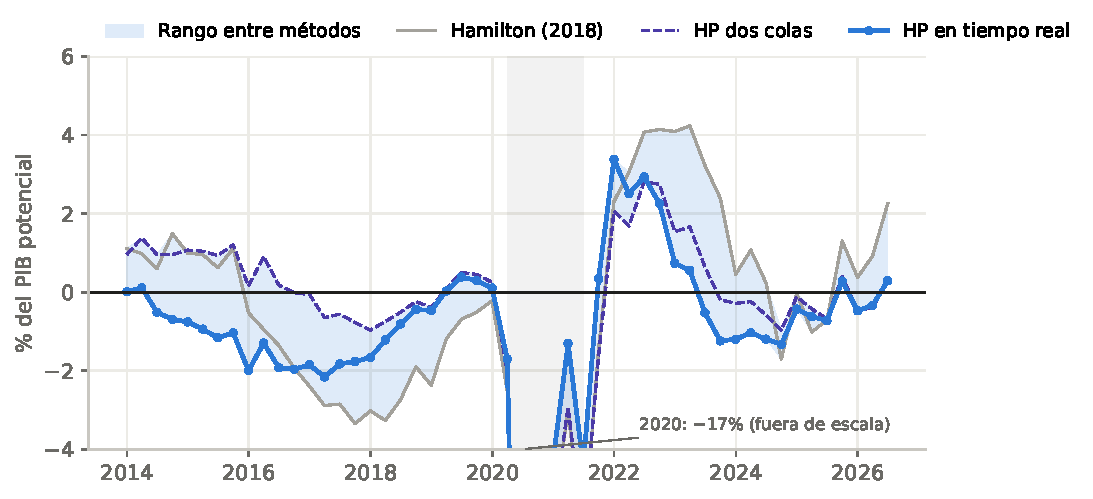
\includegraphics[width=\linewidth]{brecha_producto.pdf}
\column{0.34\textwidth}
\cifra{+0,3\%}\\
{\small brecha del producto, T2 2026}\\[0.8em]
\small Rango entre métodos: \textbf{+0,3 a +2,3}\\
Los tres métodos: brecha positiva\\
PIB real +3,5\% · potencial 2,4\%
\end{columns}
\fuente{DANE, PIB desestacionalizado ref. 2015. HP en tiempo real ($\lambda=1600$), HP dos colas y Hamilton (2018).}
\end{frame}

\begin{frame}{El reloj del ciclo: entrando a expansión}
\begin{columns}[c]
\column{0.5\textwidth}\centering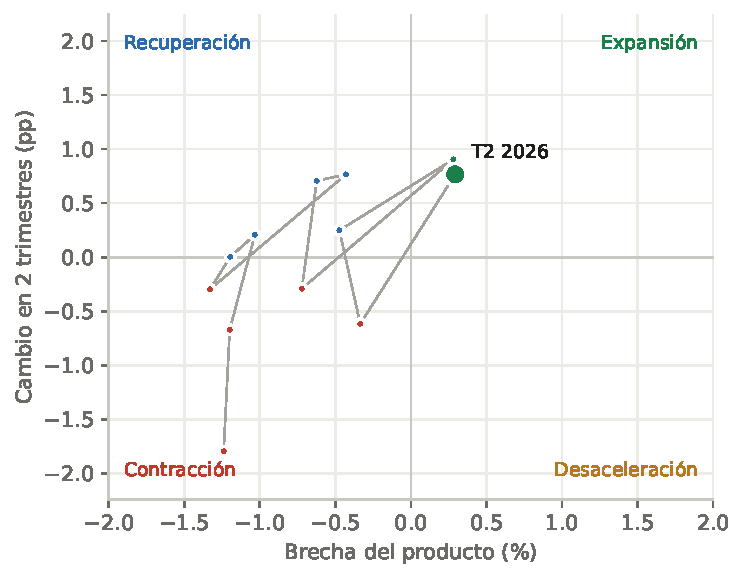
\includegraphics[height=0.72\textheight]{reloj_ciclo.pdf}
\column{0.46\textwidth}
\begin{itemize}
\item Eje horizontal: \textbf{nivel} de la brecha
\item Eje vertical: \textbf{dirección} (cambio en 2 trimestres)
\item Tras dos años en contracción/recuperación, T2 2026 cruza a \textcolor{cmgreen}{\textbf{expansión}}
\end{itemize}
\end{columns}
\fuente{Metodología del \emph{business cycle clock} de la OCDE aplicada a la brecha HP en tiempo real.}
\end{frame}

\begin{frame}{2 · Precios: la inflación se aleja de la meta}
\begin{columns}[c]
\column{0.64\textwidth}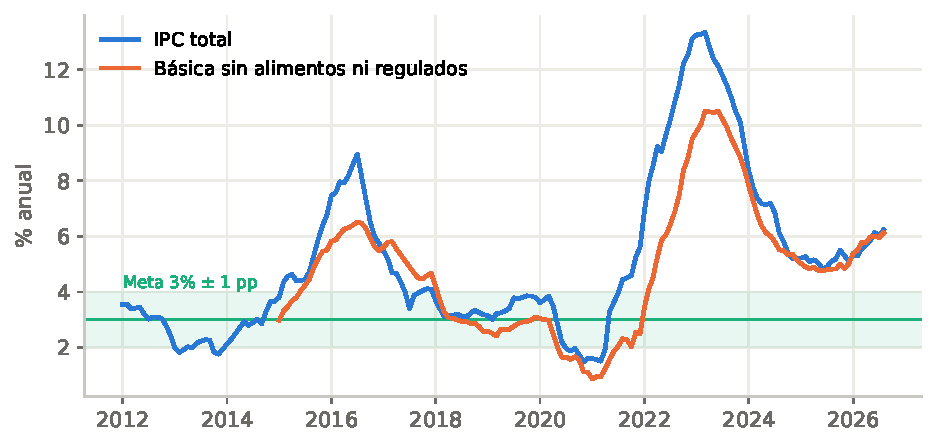
\includegraphics[width=\linewidth]{inflacion.pdf}
\column{0.34\textwidth}
\cifra{6,24\%}\\
{\small IPC anual, agosto 2026}\\[0.8em]
\small Básica sin alimentos ni regulados: \textbf{6,12\%}\\
+0,40 pp en tres meses\\
Presión \alert{generalizada}, no solo alimentos
\end{columns}
\fuente{DANE; BanRep serie 15390. Rango meta 3\% ± 1 pp.}
\end{frame}

\begin{frame}{El mercado no espera convergencia pronto}
\begin{columns}[c]
\column{0.64\textwidth}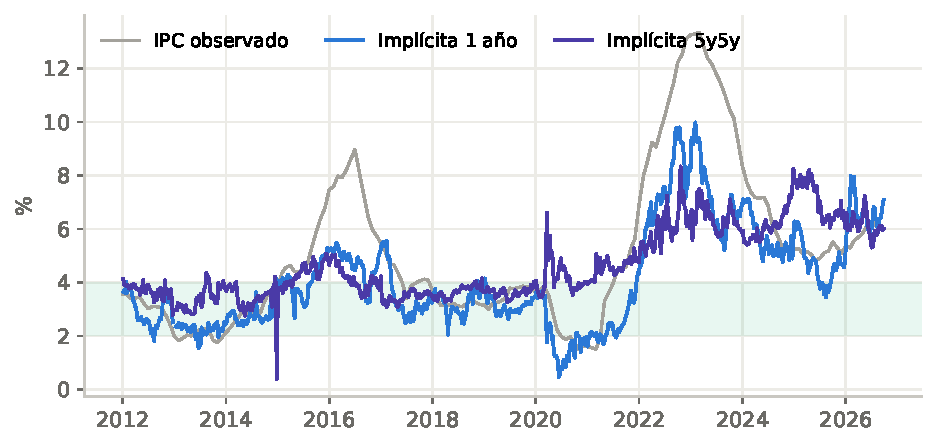
\includegraphics[width=\linewidth]{expectativas.pdf}
\column{0.34\textwidth}
\cifra{6,0\%}\\
{\small inflación implícita 5y5y}\\[0.8em]
\small A 1 año: \textbf{7,1\%}\\
El techo del rango es 4\%\\
Expectativas \alert{desancladas}
\end{columns}
\fuente{$\pi^{BE}_h=(1+i^{COP}_h)/(1+r^{UVR}_h)-1$ con curvas cero cupón TES (BanRep). Incluye primas de riesgo y liquidez.}
\end{frame}

\begin{frame}{3 · Política: postura claramente restrictiva}
\begin{columns}[c]
\column{0.64\textwidth}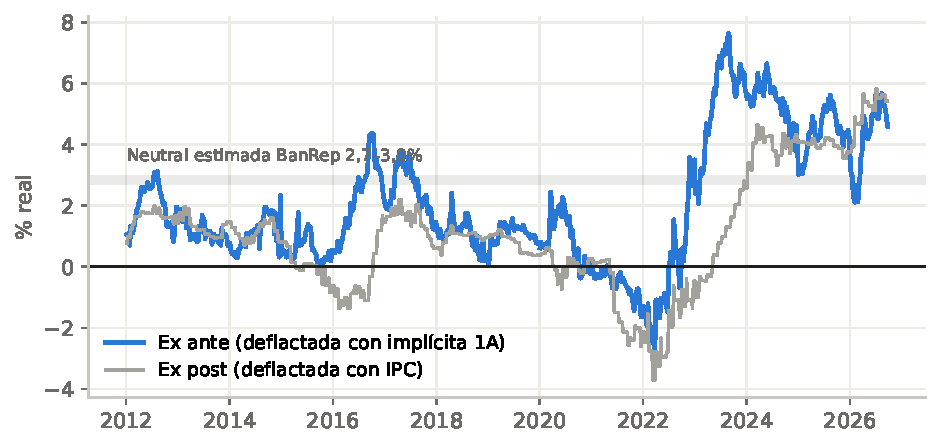
\includegraphics[width=\linewidth]{tasa_real.pdf}
\column{0.34\textwidth}
\cifra{4,6\%}\\
{\small tasa real ex ante}\\[0.8em]
\small Tasa de política \textbf{12,0\%}\\
Neutral estimada 2,7–3,0\%\\
Tres alzas en 2026 (9,25 $\rightarrow$ 12,0)
\end{columns}
\fuente{$r^{ea}=(1+TPM)/(1+\pi^{BE}_1)-1$. Neutral: estimación del equipo técnico de BanRep (2025).}
\end{frame}

\begin{frame}{La curva TES subió en todos los plazos}
\begin{columns}[c]
\column{0.52\textwidth}\centering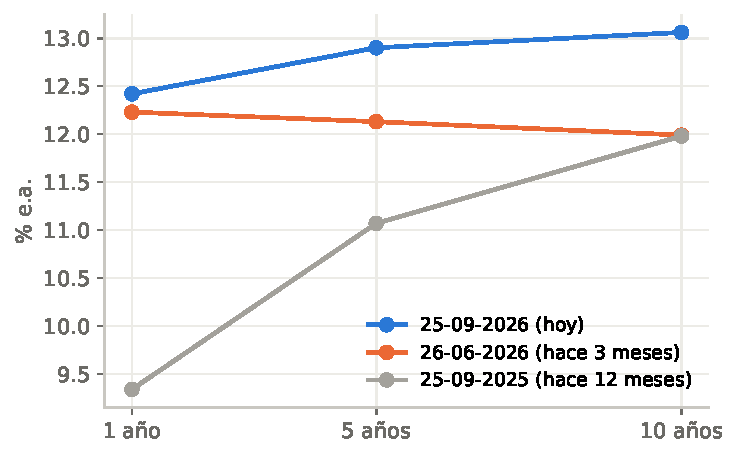
\includegraphics[width=\linewidth]{curva_tes.pdf}
\column{0.44\textwidth}
\begin{itemize}
\item TES 10 años: \textbf{13,06\%} (percentil 96 desde 2010)
\item Pendiente 10A–1A: \textbf{+0,64 pp}, casi plana
\item El mercado exige prima alta a todos los plazos
\end{itemize}
\end{columns}
\fuente{BanRep, curvas cero cupón TES pesos (Nelson–Siegel).}
\end{frame}

\begin{frame}{4 · Mercados: rally bursátil amplificado por el peso}
\begin{columns}[c]
\column{0.64\textwidth}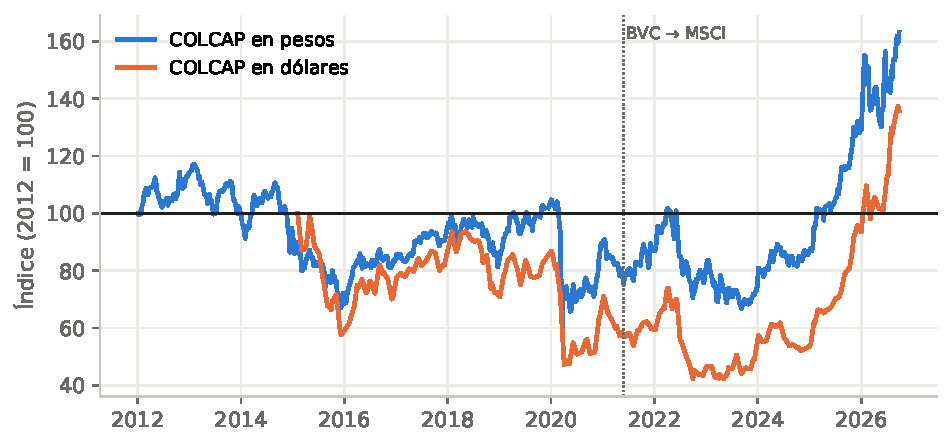
\includegraphics[width=\linewidth]{colcap.pdf}
\column{0.34\textwidth}
\cifra{+38,7\%}\\
{\small COLCAP en 12 meses (pesos)}\\[0.8em]
\small Más en dólares por la apreciación del peso\\
Tasa de cambio real en mínimo histórico\\
Cuenta corriente −3,5\% del PIB
\end{columns}
\fuente{BanRep (BVC/MSCI COLCAP; TRM). Índice de precios: no incluye dividendos.}
\end{frame}

% ---------------------------------------------------------------- 13
\begin{frame}{La lectura integrada}
\begin{center}
\begin{tabular}{@{}lll@{}}
\toprule
\textbf{Bloque} & \textbf{Dato} & \textbf{Lectura}\\\midrule
Actividad & Brecha +0,3\% (rango +0,3 a +2,3) & \textcolor{cmgreen}{Expansión}, cerca del potencial\\
Precios & IPC 6,24\% · básica 6,12\% & Acelerando, fuera del rango\\
Expectativas & 1 año 7,1\% · 5y5y 6,0\% & Desancladas\\
Política & Real ex ante 4,6\% & Restrictiva\\
Mercados & TES 10A 13,06\% · COLCAP +38,7\% & Prima alta, bolsa fuerte\\
\bottomrule
\end{tabular}
\end{center}
\vspace{0.6em}
\centering\small\color{cmmuted}Generado automáticamente por reglas explícitas — no es opinión editorial.
\end{frame}

\section{¿Qué tan confiable es?}

\begin{frame}{Validación: la inflación implícita sí informa}
\begin{columns}[c]
\column{0.44\textwidth}\centering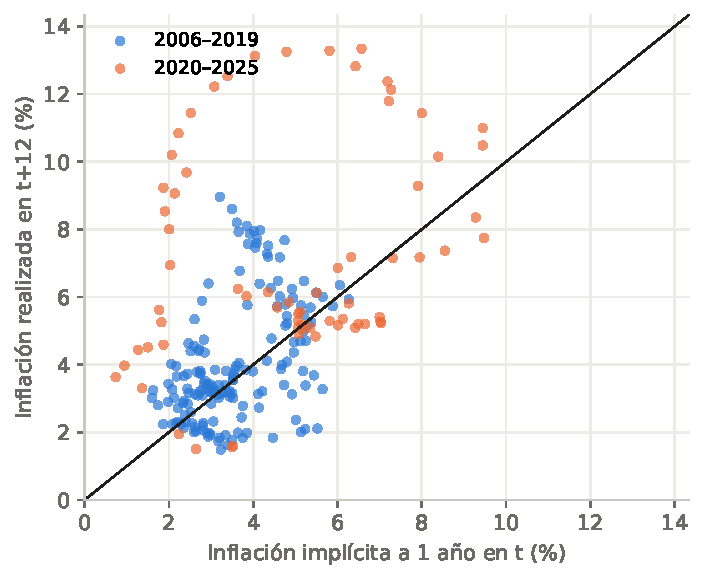
\includegraphics[height=0.74\textheight]{validacion_bei.pdf}
\column{0.54\textwidth}
\small
\begin{tabular}{@{}lrr@{}}
\toprule
 & \textbf{RMSE implícita} & \textbf{RMSE caminata}\\\midrule
2006–2019 & \textbf{1,70} & 2,08\\
2020–2025 & 4,13 & 4,07\\
Total & 2,64 & 2,80\\
\bottomrule
\end{tabular}\\[0.8em]
Antes de 2020 pronostica mejor que “la inflación no cambia”. Ningún método anticipó el choque de 2021–23.
\end{columns}
\fuente{Implícita a 1 año (promedio mensual) frente a la inflación realizada 12 meses después; 236 meses.}
\end{frame}

\begin{frame}{Robustez: el nivel es sólido, la fase es sensible}
\begin{center}
\begin{tabular}{@{}lr@{}}
\toprule
\textbf{Métrica} (51 trimestres, 2013–2026) & \textbf{Valor}\\\midrule
Mismo signo: HP tiempo real vs. HP dos colas & 78\%\\
Mismo signo: HP tiempo real vs. Hamilton & 65\%\\
Misma fase: HP tiempo real vs. Hamilton & 43\%\\
Revisión media tiempo real $-$ dos colas & $-0{,}52$ pp\\
\bottomrule
\end{tabular}
\end{center}
\vspace{0.6em}
$\Rightarrow$ Por eso el tablero muestra la \alert{banda} entre métodos y cuántos coinciden.
\end{frame}

\begin{frame}{Limitaciones que declaramos}
\begin{itemize}
\item Una sola \emph{vintage}: no reconstruimos lo que se sabía en cada fecha pasada
\item La tasa neutral es una estimación externa
\item Las implícitas contienen primas de riesgo y liquidez
\item COLCAP es índice de precios (sin dividendos)
\item Las canastas heredadas quedan en un laboratorio, fuera de las cifras
\end{itemize}
\end{frame}

\begin{frame}[c]{Demostración}
\centering
{\Large El tablero en vivo}\\[1em]
{\color{cmblue}\large github.com/Stv-Quant/ColombiaMacro-USBCali}\\[1.2em]
\small Veredicto $\rightarrow$ brecha y reloj $\rightarrow$ expectativas $\rightarrow$ tasa real $\rightarrow$ tablero de señales
\end{frame}

\begin{frame}{Próximos pasos}
\begin{columns}[T]
\column{0.48\textwidth}
\textbf{Metodología}
\begin{itemize}
\item Base de datos de \emph{vintages} del PIB
\item Nowcasting con factores dinámicos (ISE + indicadores mensuales)
\item Descomposición expectativa/prima con un modelo afín de la curva
\end{itemize}
\column{0.48\textwidth}
\textbf{Colaboración}
\begin{itemize}
\item Revisión metodológica con el equipo técnico de BanRep
\item Alojamiento institucional en la USB Cali
\item Uso docente en cursos de macroeconomía y finanzas
\end{itemize}
\end{columns}
\end{frame}

\begin{frame}[standout]
Colombia está en \textbf{expansión},\\ con inflación \textbf{fuera de la meta},\\ política \textbf{restrictiva}\\ y expectativas \textbf{desancladas}.\\[1em]
{\normalsize Cada afirmación es verificable con datos oficiales.}
\end{frame}

% ================================================================ apéndice
\appendix
\section*{Apéndice técnico}

\begin{frame}{A1 · Fisher, inflación implícita y 5y5y}
\[
\pi^{BE}_h=\frac{1+i_h}{1+r_h}-1,\qquad
\pi^{5y5y}=\frac{\left[(1+i_{10})^{10}/(1+i_5)^{5}\right]^{1/5}}{\left[(1+r_{10})^{10}/(1+r_5)^{5}\right]^{1/5}}-1
\]
\small Ejemplo (25-sep-2026): $i_1=12{,}42$, $r_1=4{,}99 \Rightarrow 7{,}08\%$; $f^{nom}=13{,}22$, $f^{real}=6{,}80 \Rightarrow 6{,}01\%$.
\[
r^{ea}_t=\frac{1+TPM_t}{1+\pi^{BE}_{1,t}}-1=\frac{1{,}12}{1{,}0708}-1=4{,}60\%\quad(\text{vs. }4{,}92\text{ con la aproximación})
\]
\end{frame}

\begin{frame}{A2 · Filtro HP en tiempo real}
\[
\tau=\arg\min_{\tau}\sum_{t=1}^{T}(y_t-\tau_t)^2+\lambda\sum_{t=2}^{T-1}(\Delta^2\tau_{t+1})^2
\;\Rightarrow\; \tau=(I+\lambda D^\top D)^{-1}y,\quad \lambda=1600
\]
\begin{itemize}\small
\item $y_t=100\ln Y^{sa}_t$; brecha $g_t=y_t-\tau_{t|t}$ usando solo $y_1,\dots,y_t$ (mínimo 20 trimestres)
\item Evita el sesgo de fin de muestra (Orphanides y van Norden, 2002)
\item Coincide con \texttt{statsmodels.hpfilter} hasta $2\times10^{-10}$
\item 2020-T2 a 2021-T2 interpolados \emph{solo} para estimar la tendencia
\end{itemize}
\end{frame}

\begin{frame}{A3 · Hamilton (2018) y reloj del ciclo}
\[
y_{t+8}=\beta_0+\sum_{k=0}^{3}\beta_k\,y_{t-k}+v_{t+8},\qquad \hat g^{H}_{t+8}=y_{t+8}-\hat y_{t+8}
\]
\begin{center}\small
\begin{tabular}{@{}lcc@{}}
\toprule
 & $\Delta_2 g\ge0$ & $\Delta_2 g<0$\\\midrule
$g\ge0$ & \textcolor{cmgreen}{Expansión} & \textcolor{cmamber}{Desaceleración}\\
$g<0$ & \textcolor{cmblue}{Recuperación} & \textcolor{cmred}{Contracción}\\
\bottomrule
\end{tabular}
\end{center}
\end{frame}

\begin{frame}{A4 · Fuentes}
\small
\begin{tabularx}{\textwidth}{@{}lXl@{}}
\toprule
\textbf{Bloque} & \textbf{Series} & \textbf{Fuente}\\\midrule
Actividad & PIB real ref. 2015 (Cuadros 1 y 4), ISE, GEIH desestacionalizada & DANE\\
Precios & IPC; básica 15388/15390/15392; regulados 15398; alimentos 15404; meta 853 & DANE, BanRep\\
Tasas & TES cero cupón pesos y UVR 15272–15277; TPM 59; IBR 15324 & BanRep\\
Mercados & COLCAP 6; TRM 1; ITCR 235 & BanRep (BVC/MSCI, SFC)\\
Externo y fiscal & Cuenta corriente 15290; IED 15133; reservas 15051; deuda GNC 15328 & BanRep, MinHacienda\\
\bottomrule
\end{tabularx}
\end{frame}

\begin{frame}{A5 · Reglas del veredicto y control de calidad}
\small
\begin{columns}[T]
\column{0.5\textwidth}
\textbf{Reglas}
\begin{itemize}
\item Cerca del potencial si $|g|<0{,}5$
\item Acelera si $\Delta_3\pi>0{,}1$ pp
\item Restrictiva si $r^{ea}>3{,}0+0{,}5$
\item Desancladas si 5y5y $>4\%$
\end{itemize}
\column{0.5\textwidth}
\textbf{Controles}
\begin{itemize}
\item Identidad de serie (id + nombre)
\item Rangos, fechas, frecuencias
\item Fórmulas recalculadas cada día
\item Saltos aislados excluidos y registrados
\item 43 pruebas automáticas
\end{itemize}
\end{columns}
\end{frame}

\end{document}
